\documentclass[12pt]{article}
\usepackage[dvips]{epsfig}
\usepackage{fleqn}
\usepackage{amssymb,amstext}
\usepackage{array}
\usepackage[latin1]{inputenc}
\usepackage{amsmath}
\usepackage[margin=1in]{geometry}
\usepackage{array}
\usepackage{amsmath}
\usepackage{latexsym}
\usepackage{psfrag}
\usepackage{graphicx}
\usepackage{setspace}
\usepackage{caption2}
\usepackage{url}
\usepackage{fancyhdr}
\usepackage{natbib}
\usepackage{cancel}
\usepackage{hyperref}
\usepackage{enumitem}
\usepackage{pdfpages}
\usepackage{indentfirst}
\usepackage{float}

\usepackage{pdflscape}
\usepackage{multirow}
\usepackage{longtable}

\usepackage{xcolor}

\usepackage{subfiles}
 
\usepackage{blindtext}


%\usepackage[utf8]{inputenc}

\hypersetup{
    colorlinks,
    citecolor=black,
    filecolor=[rgb]{0,0.5,0.5},
    linkcolor=black,
    urlcolor=black
}

\renewcommand\listfigurename{}
\renewcommand{\captionlabelfont}{\bf}
\renewcommand{\captionlabeldelim}{.}
\newcommand{\argmax}{\operatornamewithlimits{argmax}}
\renewcommand{\baselinestretch}{2}
\renewcommand\refname{References}
\newcommand\crule[3][black]{\textcolor{#1}{\rule{#2}{#3}}}

\setcounter{secnumdepth}{0}
\makeatletter

%\providecommand*{\input@path}{}
%\g@addto@macro\input@path{{./level1//}{./level1/level2//}{./level2//}}
%\makeatother

%\renewcommand\section{\@startsection {section}{1}{\z@}%
%                                   {-3.5ex \@plus -1ex \@minus -.2ex}%
%                                   {2.3ex \@plus.2ex}%
%                                   {\centering\normalfont\Large\scshape}}
%\renewcommand\subsection{\@startsection {subsection}{1}{\z@}%
%                                   {-3.5ex \@plus -1ex \@minus -.2ex}%
%                                   {2.3ex \@plus.2ex}%
%                                   {\normalfont\bf}}
\renewcommand*\contentsname{}                                   
\pagenumbering{gobble}                                   
\begin{document}
	
	\pagenumbering{roman}
	\begin{center}
	{\bf \Large Armillaria Gallica Gene Analysis Tools}
	\end{center}

%%%%%%%%%%%%%%%%%%%%%%%%%%%%%%%%%%%
%
%	Analysis Methods
%
%%%%%%%%%%%%%%%%%%%%%%%%%%%%%%%%%%%

\section{Methods}
This section will brief explanation of all methods used over the course of this class. For all programs discussed here see \url{https://github.com/ofbujak/Armillaria_gallica_gene_analysis_tools}.

\subsection{Read Depth Snapshots}
	The first work completed was the analysis of the read depth values for each of the 15 sequenced strains of the \textit{Armillaria gallica}. This work was based on analysis which a former student, Hao Wang, had done previously to determine locations for each strain that had unusually high read depth. These locations are based on reads aligned to a reference. Unfortunally, we do not know the exact method which Hao had used to determine which locations he had deemed had significant read depth. Though we do not know the exact method he used, the regions he identified were those that had high read depth. He outputted his results into text files consisting of three columns, a scaffold number column, a location start column, and a location end column. These files had variable numbers of locations of high significance but they averaged approximatly 2636 locations per strain. With the goal to produce graphs of these locations of high read depth, in order to gain a understainding of the "landscape" about those locations, I first made up of the samtools \textit{depth} command in a program called make\_read\_depth\_files.sh

make\_read\_depth\_files.sh will output a file which has three columns, scaffold, location, and read depth. Using these results I wrote a program, read\_depth\_per\_location.c, which will take in as arguments a specific samtools read depth file, a scaffold to search for, a start and end location (all space separated). read\_depth\_per\_location.c will then print information (scaffold, location, read depth, etc...) on the locations, incrementing by 1 from the start location, for all locations which are within the range passed into it. This program was used in plot\_all\_read\_depths.sh to produce graphs of each range of locations with high read depth $\pm$ 500. The program used to create the graphs was plot\_read\_depth.R. Some examples of these graphs can be found in figures \ref{avg_rd_snpsht_1} and \ref{avg_rd_snpsht_2}.
	
\subsection{Read Depths For Whole Scaffolds}
	In order to produce depictions of the read depths for an entire scaffold the framework established to create the read depth snapshots was used with some slight changes in methodology. To produce these graphs the files produces from using the samtools \textit{depth} command were searched via grep in order to separate each scaffold result into its own file. These files were then passed into plot\_scaffold\_read\_depth.R and plot\_scaffold\_read\_depth\_histogram.R. plot\_scaffold\_read\_depth.R is a program which graphs the read depth on the y axis and the location of that read depth on the x axis. plot\_scaffold\_read\_depth\_histogram.R creates a histogram of the read depths with binwidths of 5. %The results for these section can be found in section \ref

\subsection{Read Depth Analyses}
	In order to gain insight into the different aspects of the scaffolds and the reads which were aligned I produced four metrics for each strain. I calculated the global average read depths, determined the total number of sites with reads aligned to them, calculated and graphed the average number of reads per scaffold, and graphed and determined the number of locations with reads aligned for each scaffold. 

\subsection{Unaligned Reads}
	To output all reads which are not aligned into a sam file the following samtools view command can be used: samtools view -f 4 file.bam $>$ unmapped.sam. Following this The reads can be assembled via a de novo assembler. (The assembly of these has not been carried out yet).

\subsection{New Assemblies}
	To produce new assemblies I attempted to do both \textit{de novo} assemblies of five of the strains (Ar170, Ar174, Ar179, Ar196, Ar213). Following verification of quality using FastQC, both methods were used.

	\subsubsection{De Novo Assemblies}
	To produce new \textit{de novo} assemblies of five of the strains (Ar170, Ar174, Ar179, Ar196, Ar213) were attempted. The program used for the assmeblies was Velvet, with the wrapper VelvetOptimiser used. The command used to run VelvetOptimiser was: 
\begin{verbatim}
'perl VelvetOptimiser.pl -f "-shortPaired -fastq -separate 
<Path To Forward Strand File>/<Forward_strand.fastq.gz> 
<Path To Reverse Strand File>/<Reverse_strand.fastq.gz>" -t 32 -s 31 -e 31 
-d <Output Directory>
\end{verbatim}

	\subsubsection{Reference Based Assemblies}
	`To produce another reference based assembly the scipt fastqThroughNovoalign.sh was used. Due to time constraints, the reference based assemblies have not been analyzed as of yet.

\subsection{Taking the Consensus of Aligned Read}
	Following identification of locations where read depth is significant it was useful to be able to quickly get the actual DNA sequence which is aligned to a specific location. To do this, custom programs were created to sort through the output from samtools view and to take the consensus of the reads aligned. The total pipeline for these programs is encapsulated within consensus\_reads.sh.
	
	To output sequences that were easier to work with, samtools view was used. The command used was: \begin{verbatim}samtools view -o <output_filename> <bam_file> 
<scaffold_number>:<location_start>-<location_end>\end{verbatim} . This command created a sam file with 11 columns (these columns are explained in the file SAMv1.pdf found in Extra_Documents), five of which are required for the following programs. The five required are: the scaffold or contig which a read is aligned to, the location which the first base in a read is aligned to, the cigar string (\textbf{C}ompact \textbf{I}diosyncratic \textbf{G}apped \textbf{A}lignment \textbf{R}eport) which give information about what bases from the read align to the reference, the actaul read itself, and the quality score for each base in the read. 

	Following outputting of the sam file, the program 'pull\_reads.c' is used. This program takes in the five columns listed above (in the order discussed) and outputs all the reads, which fall within the range specified, into a file where each read occupies its own line with each read offset by the difference between the start of the range of interest and the location which the read starts.
	
	The output created by pull\_reads.c is then passed into average\_reads.c. average\_reads.c takes in the output created by pull\_reads.c and the difference between the start and end locations. This program creates 4 arrays of the size of the difference passed into the program and iterates over all lines in the file. When a base is encounteres at a location the array for that base is incremented by 1, at the location of that base. After all the lines in the file are iterated over, the mode of each base for each element of the array are then output, resulting in a consensus of the reads that were aligned between two locations.

\subsection{Calculation of Average Read Depth and Number of Aligned Reads per Scaffold}
	The program avg\_read\_depth.c takes in a read depth file and the scaffold which the average of which will be calculated and outputs the average read depths for the locations with reads aligned to them and the total number of locations with reads aligned to them for that scaffold.

\subsection{Determiation of Regions Of High Read Depth}
	To create a new method for deremining the regions of the assembly which had significant read depth high\_read\_depth\_regions.c was created. This program takes in the average number of reads aligned to a scaffold, and the number of locations on a scaffold with reads aligned, and searches for all locations with read depth higher than a certian threshold. The threshold used for these analyses was a multiple of five fold the standard deviation plus the mean. Any regions which were found to be above that were identified as having significant read depth. In addition to the search this program also allows for a 10 base grace peroid. If a region was found to have significant read depth had some locations immediatly following it which were below the threshold for less than 10 consecutive locations before the read depth rose above the level of significance than the entire region, including the up to 10 bases below that region would be reported as once contigious region of high read depth.

\subsection{Compairisons of Read Depths}
	The program compare\_read\_depths.c takes in two read depth files, a reference file and a compairison file. This program iterates over all the lines in the file and comapires each location and calculates the difference between read depths.

\subsection{Analysis of DNA Sequences Suspected to Result in High Read Depths}
	Using the locations found to have significant read depth and the method used to take the consensus of the the aligned reads between locations, the sequences at each location which had high read depth could be extracted. After these sequences were extracted they could be searched, via ncbi blastn, to attempt to determine if the sequence has any homologous in other species/ to determine the effect of the sequence.


\subsection{Insertions and Deletions}

	Kassandras stuff here.


\section{main}
All the stuff Thomas did:
\begin{itemize}
	\item read depth snapshots - check!
	\item average read depth stuff
	\item total number of aligned reads
	\item program to take mode of reads
	\item scaffold graphing program
	\item read depth differences program
	\item assemblies
	\item blasting stuff
	\item RNA verification
\end{itemize}
%%%%%%%%%%%%%%%%%%%%%%%%%%%%%%%%%%%
%
%	Read Depth Snapshot
%
%%%%%%%%%%%%%%%%%%%%%%%%%%%%%%%%%%%
\section{Read Depth Snapshots}
	In order to gain a understanding of how the locaitons which Hao had determined had notably high read depth the regions Hao identified were graphed. There were approximatly between 2000 and 4000 regions for each of the 15 strains. Although there were many graphs four predomanant types of high read depth regions stood out: Normal, Rectangular, Right skewed, and Left skewed.
\begin{figure}[H]
	\begin{centering}
		\resizebox{40mm}{40mm}{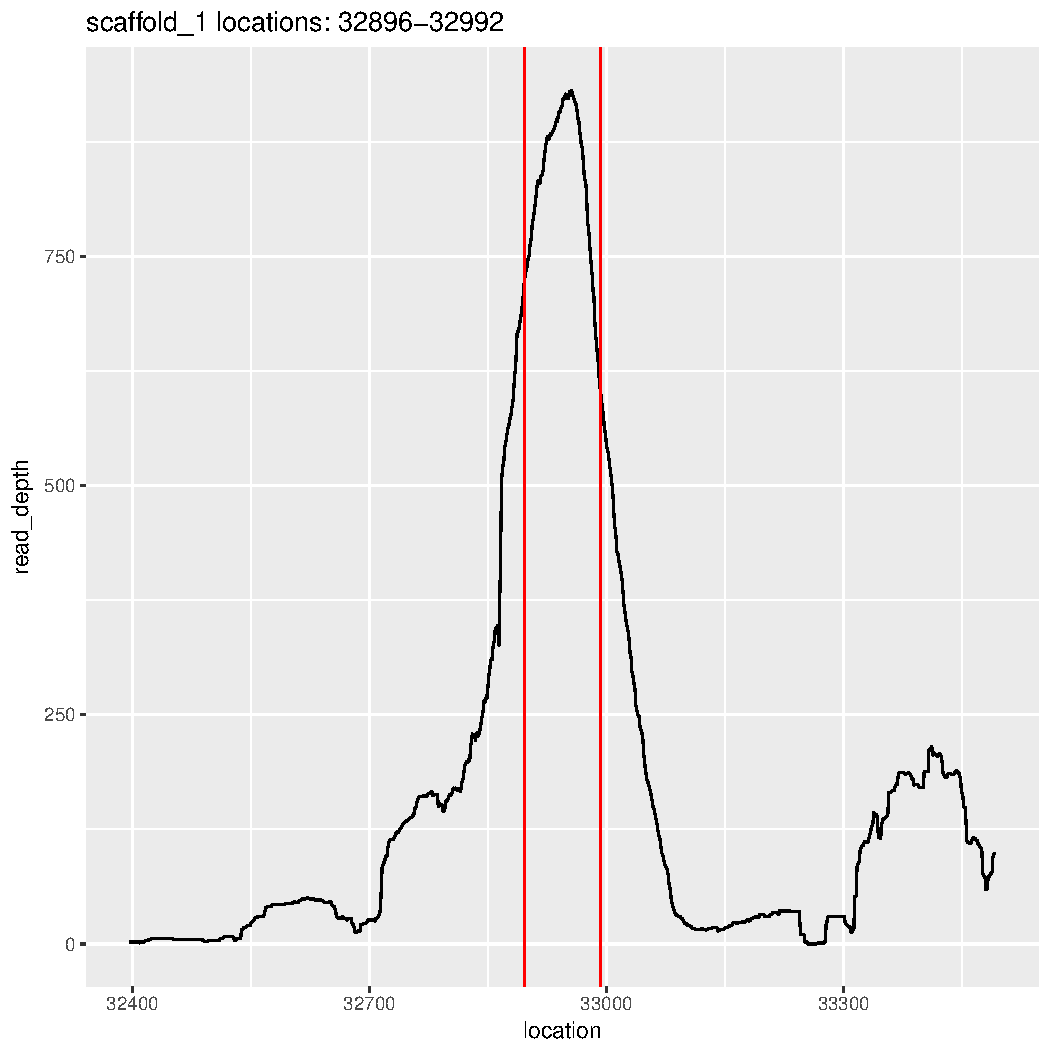
\includegraphics[angle=0,width=1.0\linewidth]{/home/thomas/Directed_Studies_Summer_2019/Armillaria_gallica_gene_analysis_tools/Reporting_documents/Figures/read_depth_snapshot_images/ctj/0_Ar109_read_depth.pdf}}
		\resizebox{40mm}{40mm}{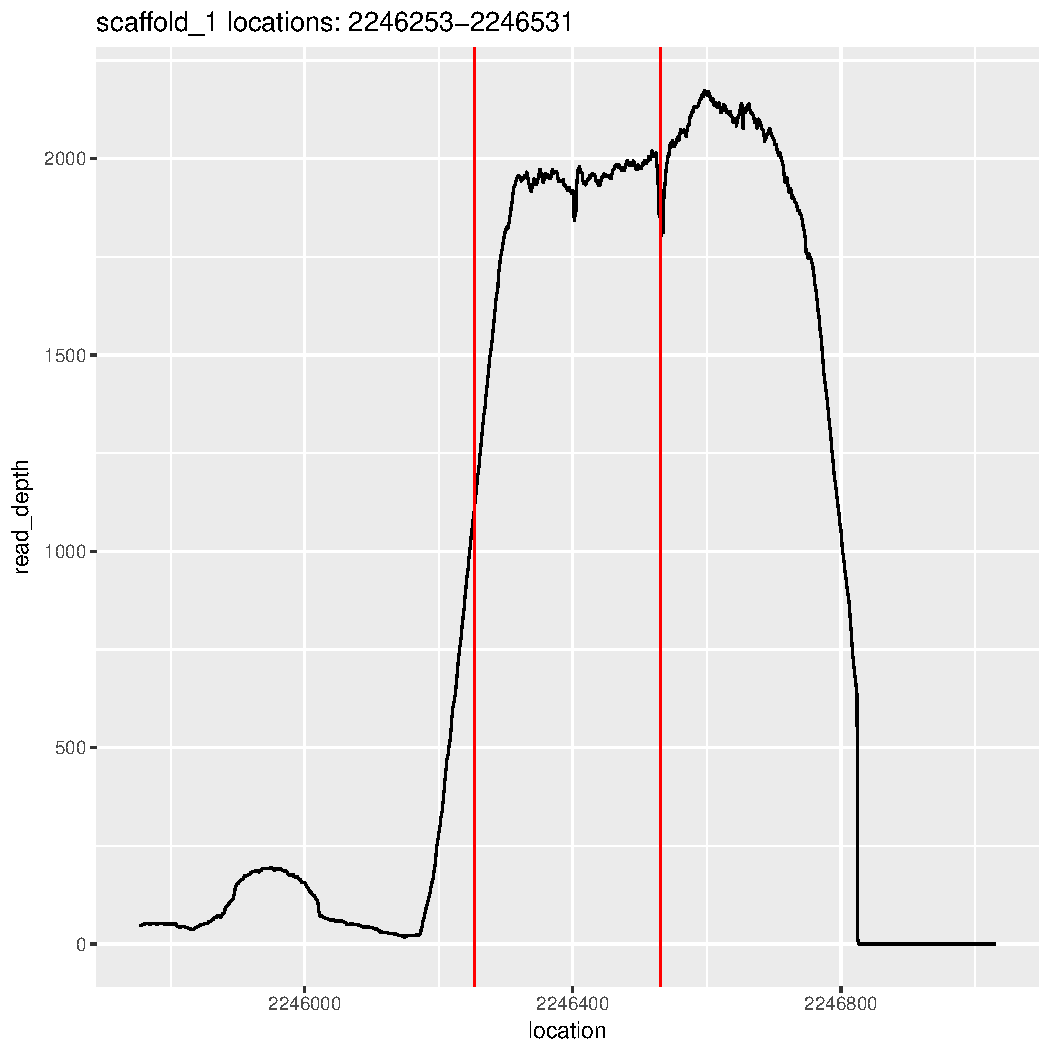
\includegraphics[angle=0,width=1.0\linewidth]{/home/thomas/Directed_Studies_Summer_2019/Armillaria_gallica_gene_analysis_tools/Reporting_documents/Figures/read_depth_snapshot_images/ctj/5_Ar109_read_depth.pdf}}
		\resizebox{40mm}{40mm}{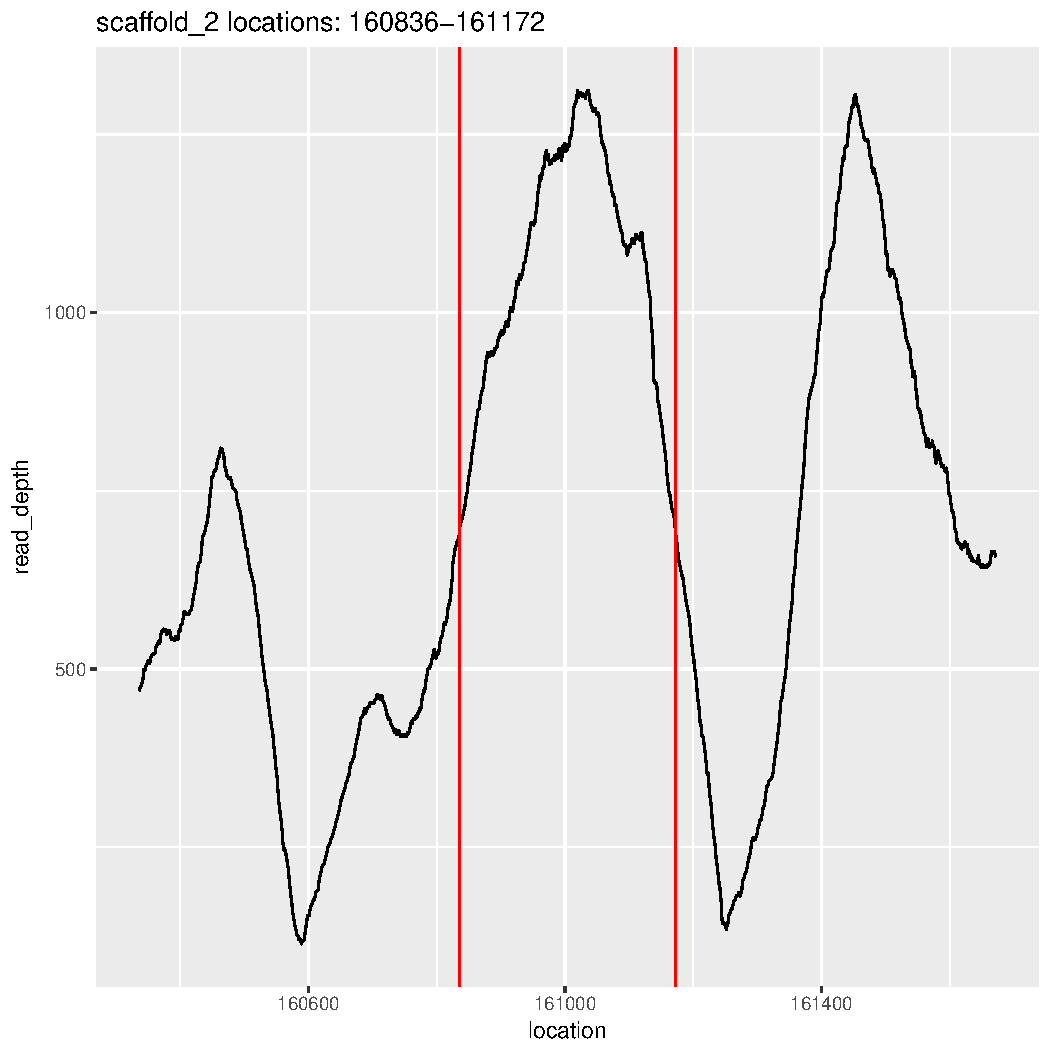
\includegraphics[angle=0,width=1.0\linewidth]{/home/thomas/Directed_Studies_Summer_2019/Armillaria_gallica_gene_analysis_tools/Reporting_documents/Figures/read_depth_snapshot_images/ctj/155_Ar109_read_depth.pdf}}
		\resizebox{40mm}{40mm}{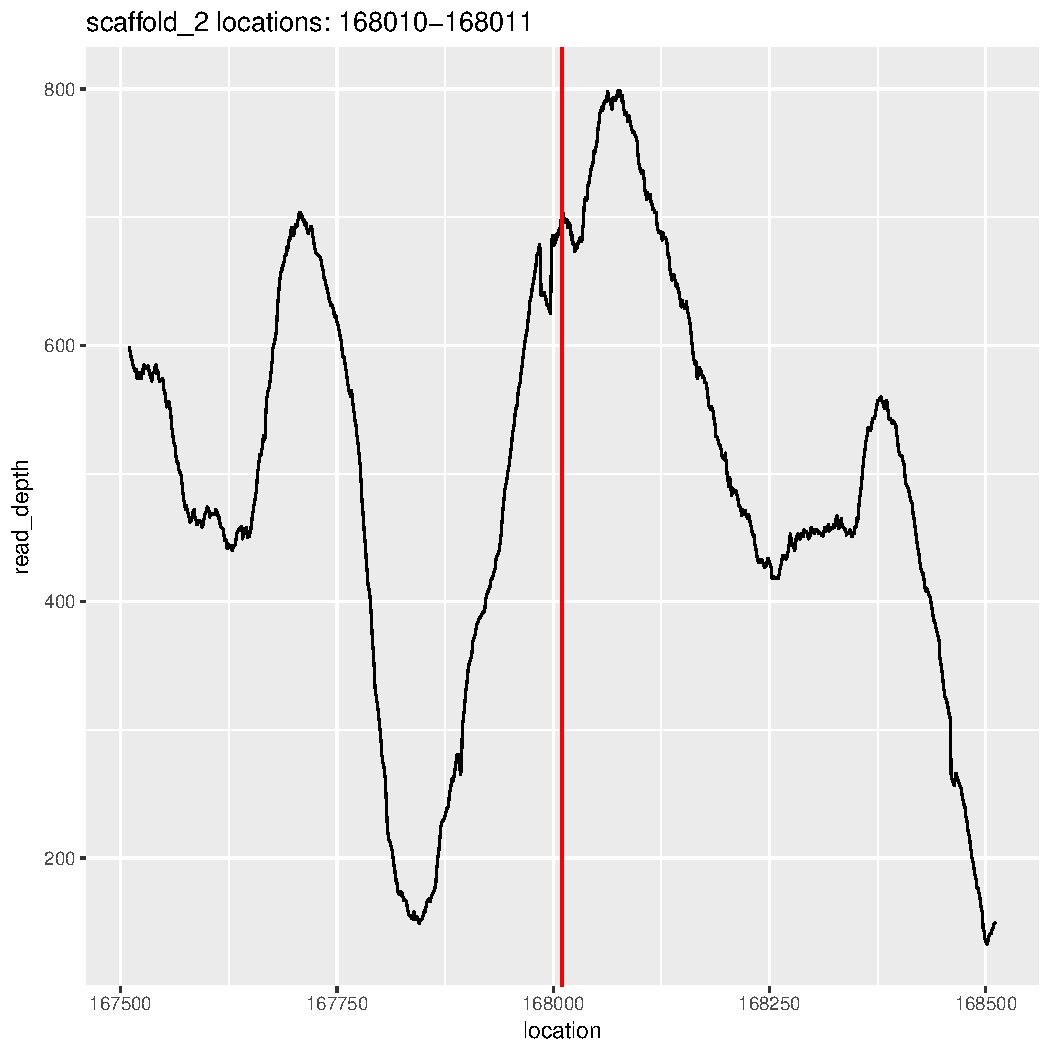
\includegraphics[angle=0,width=1.0\linewidth]{/home/thomas/Directed_Studies_Summer_2019/Armillaria_gallica_gene_analysis_tools/Reporting_documents/Figures/read_depth_snapshot_images/ctj/173_Ar109_read_depth.pdf}}
		\begin{singlespace}
			\vspace{-0.5cm}
			\caption[Examples of the four types of high read depth regions.]{Examples of the four types of high read depth regions (left most) Normal, (left middle) Rectangular, (right middle) Left skewed, (right most)Right skewed}\label{four_rds}
		\end{singlespace}
	\end{centering}
\end{figure}

%%%%%%%%%%%%%%%%%%%%%%%%%%%%%%%%%%%
%
%	Average read depth and total number of reads aligned per scaffold
%
%%%%%%%%%%%%%%%%%%%%%%%%%%%%%%%%%%%
\section{Average Read Depth}
	Due to the large quantity of data present in each bam or fastq file we had to make use of the 
%%%%%%%%%%%%%%%%%%%%%%%%%%%%%%%%%%%
%
%	Read Depth Analyses
%
%%%%%%%%%%%%%%%%%%%%%%%%%%%%%%%%%%%
	\section{Read Depth Analyses}
	%\subfile{Document_Sections/average_read_depths.tex}
	\newpage

%%%%%%%%%%%%%%%%%%%%%%%%%%%%%%%%%%%
%
%	Unaligned Reads
%
%%%%%%%%%%%%%%%%%%%%%%%%%%%%%%%%%%%
	\section{Unaligned Reads}	
	%\subfile{Document_Sections/unaligned_reads.tex}
	\newpage

%%%%%%%%%%%%%%%%%%%%%%%%%%%%%%%%%%%
%
%	Indel Analysis
%
%%%%%%%%%%%%%%%%%%%%%%%%%%%%%%%%%%%
	\section{Indel Analysis}
	%\subfile{Document_Sections/armg_indels.tex}
	\newpage

%%%%%%%%%%%%%%%%%%%%%%%%%%%%%%%%%%%
%
%	Future Directions
%
%%%%%%%%%%%%%%%%%%%%%%%%%%%%%%%%%%%
	\section{Future Directions}
	%\subfile{Document_Sections/future_directions.tex}
	\newpage
	
	\bibliography{main}
	\bibliographystyle{linquiry2}

\end{document}
